\documentclass[12pt]{article}
\usepackage{amsmath, amssymb}
\usepackage{amsthm}
\usepackage{hyperref}
\usepackage{MnSymbol}
%%\usepackage[pdftex]{graphicx}
\usepackage{enumerate}
\usepackage{amsmath}
\usepackage{amssymb}
\usepackage{multicol}
\usepackage{algpseudocode}
\usepackage{algorithm}


\usepackage[final]{graphicx}
\usepackage{subcaption}
\renewcommand{\phi}{\varphi}
\newcommand{\rarrow}{\rightarrow}
\usepackage{ listings}
\title{COMP 557: Homework 1}

\author{Guangyuan Yu(gy12)}
%Replace Partner 1 and 2 with your names.

\begin{document}
\maketitle


\section{1 Modelling sentence segmentation as search}
\subsection{1.1 Suppose our goal is to minimize the number of words in the output segmentation. Construct a deterministic state space model for this task}

For a specific compressed sentence, a state is a list of words, each of which represent a word we found so far. The order of words are the same as they appear in the sentence. Of course the words have to be in the order as in the compressed sentence.

The start state is an empty list, which means we haven't find any word. 
The action is : start from the current compressed sequence as the first character , find a word in the dictionary. If you go through all the possibilities, a specific character may have several actions. Like "sunday" has action "sunday" and "sun", if both words exist in the dictionary. 

When a valid word is found, you get to a successor state. And you start to search from one of the new remaining sequences. 

We break the search when we can't match the sequence with the dictionary or we finished matching all the word in the dictionary. In the first case, we didn't get a reasonable segmentation of the sequence. 

Goal test: If the remaining sequence is empty, we reach the goal state. 

Cost: Each step we find one more word in the sequence. We
use the number of word to represent cost. So each step has a cost of 1.

\subsection{Which search algorithms among BFS, DFS, UCS, $A*$, Bellman-Ford would produce a minimum cost path for your model and why?}
Except the DFS, all others works well. DFS can get one possible segmentation, but it is less-likely to be the shortest one. Other method find all states with one word, then search all states with two words,..., so the first segmentation would be the minimum number segmentation. For A*, if h==0, it is UCS. We could use the length of the remaining sequence as the h.




\subsection{1.3 If our goal is to maximize the number of words in the segmentation, revise the state space model from above.}
We use  $ - 1 \times (\text{number of words})$ to represent the cost. More words lead to
lower total cost. The cost of one action is changed from 1 to -1. Others stay the same as before. 
DFS and BFS  can not find optimal solutions. 
For a negative cost, A* need a good
heuristic function to hold the triangle rule. So algorithms that works for our model are: UCS, A*, Bellman-Ford.

\subsection{1.4Modify the state space model from above to find the
most fluent segmentation.}

Cost: 
For the first found word, cost is 0. From the second found word, its cost is
the $$fluence(\text{last found word}, \text{current found word}) $$. 
The goal state is still a goal state with minimum total costs. 
BFS, Bellman-Ford, UCS ,A* all works.




\section{2 Problem 2}

\subsection{}
Admissible heuristic:
For a point $n$ from start $s$ to destination $t$, its heuristic is:
\begin{equation}
   h(n) = \cfrac{G(n,t)}{S_H}
\end{equation}
where $G(n,t)$ is the distance between two points along the surface of the
earth. Since $G(n,t)$ is the shortest path possible between nodes $n$ and $t$ and
$S_H$ is the maximum speed, we can know that $h(n)$ is the minimum
driving time from $n$ to $t$.

\subsection{}
Consistent heuristic:
For a point $n$ from start $s$ to destination $t$ with landmark $L$, its heuristic is:
\begin{equation}
h(n) = abs(T(n,L) - T(t,L))
\end{equation}
while T(n,L) is the amount of time it takes to get from node n to landmark L.

\subsection{}





Since $h_1$ and $h_2$ are consistent heuristics, we have:
\begin{align*}
h_1(s) & \leq c(s,a,s') + h_1(s') \\
h_2(s) & \leq c(s,a,s') + h_2(s') \\
\end{align*}
Hence we have
\begin{align*}
h(s) & = \max(h_1(s), h_2(s))  \\
 & \leq \max\left[ c(s,a,s') + h_1(s'), c(s,a,s') + h_2(s')\right] \\
& = c(s,a,s') + \max\left[ h_1(s'), h_2(s')\right] \\
& = c(s,a,s') + h(s')
\end{align*}
So h(s) is consistent.

\subsection{}
Since 
$h(s)  = \max(h_1(s), h_2(s))$ is still consistent,

\begin{align*}
h(s) & = \max(h_1(s), h_2(s), h_3(s),....,h_K(s))  \\
 &  =  \max\left[ \max(h_1(s), h_2(s)), h_3(s),....,h_K(s)  \right] \\
 &  =  \max\left[ \max(h_{(k+1)}(s), h_3(s)),....,h_K(s))  \right] \\
& = h_n(s)
\end{align*}

Hence maximum value of a series of consistent heuristic is still consistent.

For a point n from start s to destination t with landmark L, its heuristic is:
\begin{equation}
h(n) = \max(|T(n,L_1) - T(t,L_1)|, |T(n,L_2) - T(t,L_2)|, \ldots ,|T(n,L_K) -
T(t,L_K)|)
\end{equation}
while $T(n,L_K)$ is the amount of time it takes to get from node n to landmark
$L_K$.

\subsection{}

If new edges are added, ${h}$ might NOT remain consistent for the new model. 

For example, let's talking about  a system with three node s, s' and t. the cost(s,s'),h(s),h(s') holds the consistence in triangle. Now you adding a new shortcut which could make cost(s,s') extremely small and h(s),h(s') unchanged. Right now, they couldn't hold the triangle rule anymore. 

 
If edges are removed, ${h}$  remains consistent for the new model. After removing a edge, the cost (s,s') can only increase, which makes the triangle rule good. 


\section{Package Delivery}
	\subsection{3.1a}
		

	
	Exploring A with pastCost 0
  Action B => B with cost 0 + 4.0
  Action C => C with cost 0 + 8.0
Exploring B with pastCost 4.0
  Action C => C with cost 4.0 + 3.0
Exploring C with pastCost 7.0
numStatesExplored = 3
totalCost = 7.0
actions = ['B', 'C']
	\subsection{3.1b}
	it passed the test in grader.
	\subsection{3.2a}
			State space: position of truck ${(x, y)}$ with a list of status for each package ${[s_0, s_1, ... s_n]}$\\
		
		The initial state is initial position of truck ${x_0, y_0}$ with status of all packages are `ready':[`ready', `ready', ..., `ready']\\
		
		the goal state is initial position of truck ${x_0, y_0}$, status of all packages are `done': [`done', `done', ..., `done']\\
		
		The actions are: `Dropoff', `Pickup', `north', `south', `west', `east'\\
	
		The costs is: if the action is `north', `south', `west', or `east', cost is 1 + the number of packages carried by the truck ; if the action is `Pickup' or `Dropoff', the cost is 0. \\
		
		There are ${mn}$ possible positions for a truck. For each package, there are three statuses: `ready', `transit' and `done'. Thus, the possibilities are ${mn\*k^3}$\\
	
	\subsection{3.2b}
	it tells me 61 NUMBER OS STATES, EXPLORED. and showed me the $number sign and dot$picture of the problem
	
	
	
	
	
	\subsection{3.2c}
		
			52 states are explored in deliverySscenario1 by using A*
	
	\subsection{3.2d}
		
			34 states are explored in deliverySscenario2 by using A*
	
	\subsection{3.2e}
		
			56 states are explored in deliverySscenario3 by using A*

\section{4.Protein Folding}
	\subsection{}
		
		The state space is the current conformation ${c_i}$: $[c_{1i}, c_{2i}, c_{3i}, ... c_{(n-1)i}]$\\
	
		The initial state is a conformation ${c_0}$: $[c_{10}, c_{20}, c_{30}, ... c_{(n-1)0}]$ \\which has "i"inside the hydrophilic sequence.\\
		
		The goal state is for a specific current conformation ${c_i}$: $[c_{1i}, c_{2i}, c_{3i}, ... c_{(n-1)i}]$, its energy is less than all its neighbors. \\
		
		The cost is we use local search to find which step should go next. Change the position of "i" in the continuous sequence. 
		
		Successor: after getting the minimum cost ${cost_{ij}}$ of current state's neighbors, return the transform ${c_{ij}}$ corresponded to that minimum cost as the successor. 
		
		\subsection{}
		\paragraph{}
		Local search is suitable for solving the problem of find minimal free energy configurations, it is not good idea to go through all the possible configuration because of course some deformation will lead to a higher energy. The problem of local search is it will get the local minimum so we need to simulate for a large time. But, by a good initalization method we can get a good start. Since the hydrophilic and hydrophobic sequence are next to each other, we can fold the hydrophilic sequence to reduce the energy. Where to fold the  hydrophilic gives variation for different search. 
		
		\subsection{}

		\paragraph{}	
			1. Time complexity is O${(3^n\*n^2\*k)}$ For each node, there are 3 possible new formation, for every kind of formation, to calculate the energy, we need $n^2$, and k is the search step to get a minimum.
			
		\paragraph{}
			2. Space complexity is O${(n)}$ because we update the conformation frequently and reuse the space for it. 
		\paragraph{}	
			3. It is local search, no guaranteed to find the optimal solution. But with large amount of simulation and good initialization , it has large possibility to find the global minimum. 


\begin{lstlisting}
pseudocode
Initialize the sequence for the given amino acid.
Generate the initial conformation by folding inside
 the hydrophilic sequence. 
(Every continuous hydrophilic sequence at most 
have one "i" inside. It is from a random number generator. Usually the hydrophobic sequence 
do not fold, but if the continuous hydrophobic sequence 
is too long, then we can fold it. The definition of too 
long is : the number inside this continuous hydrophobic
 sequence> average group length. 
 The average group length = 
 total number of amino acid/number of hydrophobic sequence.)
best500erergy = calculate energy
best500sequence = initial sequence
For 500 times:
if the initial folding is self-avoiding, get another one until it is valid.
lowenergy = calculate energy
bestsequence = initial sequence

	for the link in the sequence:
		for the other 3 choices:
			get the new folding pattern
			calculate energy
			if new energy<lowenergy:
				lowenergy = new energy
				best sequence = this new sequence
if lowenergy<best500erergy:
best500erergy = lowenergy
best500sequence = best sequence		
draw the picture
				
			



\end{lstlisting}
\subsection{4.4}
I get the result by large amount of simulation. 
The result is similar to Fig2 B. By large amount of simulation it get a similar result. But this is not a good method. I didn't make the initialization successful. The method didn't find exactly the Fig 2b, it is because there is a small barrier between the two states that lead to the failure to find a best sequence.\begin{figure}[H]
  \caption{center}
  \centering
    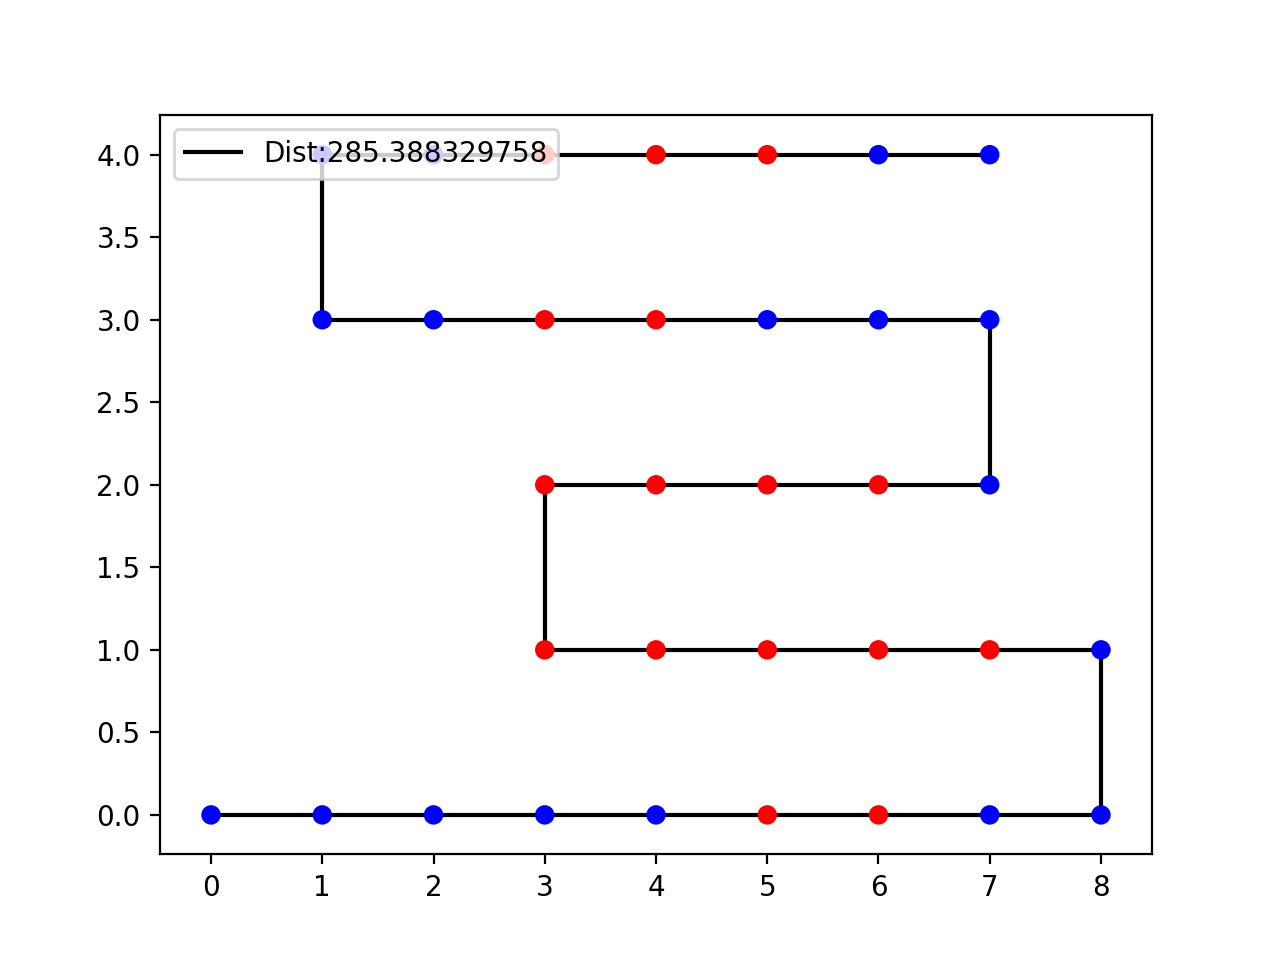
\includegraphics[scale=0.5]{figure_1.png}
\end{figure}


\end{document}

